\documentclass[11pt]{beamer} % mathserif for normal math fonts.
\usefonttheme[onlymath]{serif}
\usepackage[utf8]{inputenc}
\usepackage[swedish,english]{babel}
\usepackage{microtype}
\usepackage{calc}
\usepackage{amsmath,mathtools,dsfont}
\usepackage{contmech}
%\usepackage{siunitx}
%\usepackage{movie15}
\usepackage{multimedia}
\usepackage{grffile}
\usepackage{tikz}
\usepackage{pgfplots}
%\usepackage{subfig}

%\usepgfplotslibrary{patchplots}
%\usepgfplotslibrary{groupplots}
%\pgfplotsset{compat=1.3}

\DeclarePairedDelimiter{\homogenized}{\langle}{\rangle}
\newcommand{\pore}{\mathrm{pore}}
\newcommand{\particle}{\mathrm{part}}
\newcommand{\surf}{\mathrm{s}}
\newcommand{\prescribed}{\mathrm{p}}
\newcommand{\moving}{\mathrm{mov}}
\newcommand{\segment}{\mathrm{segm}}
\newcommand{\corner}{\mathrm{corn}}
\newcommand{\contact}{\mathrm{cont}}
\newcommand{\mesh}{\mathcal{M}}
\newcommand{\external}{\mathrm{ext}}
%\newcommand{\on}{\mid}
\newcommand{\surfdiff}{\tilde{\ts\nabla}}
\newcommand{\ded}{\mathrm{d}}
\newcommand{\dep}{\mathrm{p}}

\newcommand{\roughcite}[1]{\textsc{#1}}
\renewcommand{\alert}[1]{\textbf{#1}}

\setbeamersize{text margin left=.3cm,text margin right=.3cm}

\usetheme[titleflower=false]{chalmers}
\title{FE\textsuperscript{2} for Liquid-Phase Sintering with Seamless Transition from Macroscopic Compressibility to Incompressibility}
\author[Mikael \"Ohman]{Mikael \"Ohman\\Kenneth Runesson\\Fredrik Larsson}
\institute{Department of Applied Mechanics\\ Chalmers University of Technology}
\titlepageextra{ECCOMAS 2012}% session: Multiple-scale physics and computation
\date{2012-09-12}
%\footer{\insertshortauthor\ 2\textsuperscript{nd} ICMM}
\titlepagelogofile{figures/Avancez_black}

% Bibliography
%\bibliography{references_extended}

% Speeds up compilation.
% \usetikzlibrary{external}
% \tikzexternalize

\begin{document}

\section{Title page}
\begin{frame}[plain]
 \titlepage
\end{frame}

\section{Outline}
\begin{frame}
 \frametitle{Outline}

\begin{itemize}
 \item Background --- Motivation
 \item Subscale modeling
 \item Transition to macroscopic incompressibility
 \item Examples
 \item Conclusions --- Future work
\end{itemize}
\end{frame}

%%%%%%%%%%%%%%%%%%%%%%%%%%%%%%%%%%%%%%%%%%%%%%%%%%%%%%%%%%%%%%%%%%%%%%%%%%%%%%%%%%%%%%%%%%%%%%%%%%%
\section{Background}
\subsection{Process}
\begin{frame}
 \frametitle{Background --- Sintering of hardmetal}

% The sintering phenomenon on the mesoscale is driven by surface tension on the melted binder, and
% the homogenized effect of the surface tension is the so-called sintering stress.
% From the macroscopic perspective, the specimen (green body) shrinks due to this volumetric sintering stress. In the case of inhomogeneous
% initial density in the green body, the sintering can result in unwanted final deformations.

 \begin{enumerate}
  \item WC-particles in Co-matrix (binder metal)
  \item Precompaction $\rightarrow$ inhomogeneous ``green body'', porosity $\phi_0\approx$ 0.2--0.4
  \item Heating $\rightarrow$ thermal expansion, sintering driven by surface tension in melted Co, i.e. ``liquid phase sintering'' $\rightarrow$
        Fully dense final product $\phi=0$.
 \end{enumerate}
\alert{Note:} Inhomogeneous initial density may lead to defect product:\\ \textsuperscript{(i)}remaining porosity, \textsuperscript{(ii)}shape imperfection\\
\alert{Note:} Macroscopic compressibility despite \underline{assumed} intrinsic incompressibility of constituents until $\phi = 0$.
\begin{center}
 \begin{columns}
 \column{0.25\textwidth}\centering
 \begin{tikzpicture}
   \node at (0,0) {\includegraphics[width=\textwidth]{figures/sinter_1-crop.pdf}};
   \draw[red,thick,<-] (1,1) -- (1.5,1) node[right,black] {WC};
   \draw[red,thick,<-] (0.5,0.7) -- (1.5,0.5) node[right,black] {Co};
   \draw[red,thick,<-] (0.7,-0.3) -- (1.5,0) node[right,black] {pore};
 \end{tikzpicture}
 \column{0.05\textwidth}\centering
 $\xrightarrow{\text{idealized}}$
 \column{0.25\textwidth}\centering
 \includegraphics[width=\textwidth]{figures/sinter_2-crop.pdf}
 \end{columns}
 %\includegraphics[width=0.6\textwidth]{figures/fig081.jpeg}
\end{center}
\end{frame}

%%%%%%%%%%%%%%%%%%%%%%%%%%%%%%%%%%%%%%%%%%%%%%%%%%%%%%%%%%%%%%%%%%%%%%%%%%%%%%%%%%%%%%%%%%%%%%%%%%%
\subsection{Comparison}
\begin{frame}
 \frametitle{Constitutive modeling}
 Macroscopic modeling of sintering
 \begin{itemize}
  \item Complex model structure, requires many parameters --- calibration problem very ill-posed
  \item Selected references: \roughcite{Svoboda \& Riedel (1996)}, \roughcite{Mähler, Ekh \& Runesson (1999)}
 \end{itemize}

Mesoscale modeling of sintering - surface/interface tension
 \begin{itemize}
 \item Modeling of \textsuperscript{(i)}solid WC, \textsuperscript{(ii)}melt Co and \textsuperscript{(iii)}surface tension\\
  Note: Constitutive modeling refers to subscale constituents
  \item Selected references: \roughcite{Jagota \& Dawson (1988)}, \roughcite{van der Vorst (1993)}, \roughcite{Xu \& Mehrabadi (1997)}, \roughcite{Zhou \& Derby (1998)}, \roughcite{Peric \& coworkers (2006-)}, \roughcite{Steinmann (2008)}, \roughcite{Javili \& Steinmann (2009)}
 \end{itemize}

Computational homogenization - FE\textsuperscript{2}
\begin{itemize}
  \item Selected references:  \roughcite{Geers \& al.},  \roughcite{Fish \& al.},
 \roughcite{Miehe \& al.}, \roughcite{Larsson \& Runesson [adaptive multiscale]}
\end{itemize}
\end{frame}

%%%%%%%%%%%%%%%%%%%%%%%%%%%%%%%%%%%%%%%%%%%%%%%%%%%%%%%%%%%%%%%%%%%%%%%%%%%%%%%%%%%%%%%%%%%%%%%%%%%
\subsection{Theory}
\begin{frame}
 \frametitle{Surface tension on free surface and interfaces}
% \small
 \vspace{-1em}
 \begin{center}
  \scalebox{0.75}{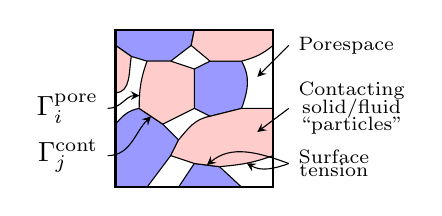
\begin{tikzpicture}[>=stealth,scale=2]
  \coordinate (A) at (0.35,0.2);
  \coordinate (B) at (0.4,0.3);
  \coordinate (C) at (0.3,0.4);
  \coordinate (D) at (0.15,0.5);
  \coordinate (E) at (0.66,0.13);
  \coordinate (F) at (0.6,0.45);
  \coordinate (G) at (0.8,0.5);
  \coordinate (H) at (0.5,0.5);
  \coordinate (I) at (0.5,0.75);
  \coordinate (J) at (0.6,0.8);
  \coordinate (K) at (0.8,0.8);
  \coordinate (L) at (0.35,0.8);
  \coordinate (M) at (0.5,1);
  \coordinate (N) at (0,0.9);
  \coordinate (O) at (0.1,0.83);
  \coordinate (P) at (0.5,0.15);
  \coordinate (Q) at (0.48,0.9);
  \coordinate (R) at (0.2,0.8);
  
  % Region 1 particles 
  \draw[fill=blue!40] 
  (0,0) -- (0.2,0) -- (A) -- (B) -- (C) -- (D) to[out=190,in=50] (0,0.4) -- cycle %A
  (0.4,0) -- (P) -- (E) -- (0.8,0) -- cycle %B
  (F) -- (G) to[out=70,in=-60] (K) -- (J) -- (I) -- (H) -- cycle %C
  (M) -- (Q) -- (L) -- (R) -- (O) -- (N) -- (0,1) -- cycle %D
  ;

  % Region 2 particles
  \draw[fill=red!20]
  (0,0.6) to[out=0,in=-100] (O) -- (N) -- cycle %E
  (D) to[out=90,in=-110] coordinate[near start] (surf3) (R) -- (L) -- (I) -- (H) -- (C) -- (D) coordinate[midway] (surf4) %F
  (M) -- (Q) -- (J) -- (K) to[out=15,in=-140] (1,0.9) -- (1,1) -- cycle %G
  (1,0.2) to[out=-160,in=5] coordinate[midway] (surf1) (E) -- (P) coordinate[midway] (surf2) -- (A) -- (B) to[out=50,in=-170] (F) -- (G) -- (1,0.5) -- cycle %H
  ;

  \draw[thick] (0,0) rectangle (1,1);

  % Annotations
  \draw[<-] (0.9,0.7) -- (1.1,0.9) node[right,font=\scriptsize] {Porespace};
  \draw[<-] (0.9,0.35) -- (1.1,0.5) node[right,font=\scriptsize] {\shortstack{Contacting\\[-0.4em]solid/fluid\\[-0.4em]``particles''}};
  \draw[<-] (surf1) to[out=-30,in=-160] (1.1,0.15) node[right,font=\scriptsize] {\shortstack{Surface\\[-0.4em]tension}};
  \draw[<-] (surf2) to[out=40,in=160] (1.1,0.15); % extra arrow
  \draw[<-] (surf3) to[out=180,in=0] (-0.05,0.5) node[left] {$\Gamma_i^{\mathrm{pore}}$};
  \draw[<-] (surf4) to[out=-135,in=0] (-0.05,0.2) node[left] {$\Gamma_j^{\mathrm{cont}}$};
\end{tikzpicture}}
  \hspace{0.5em}
  \scalebox{0.75}{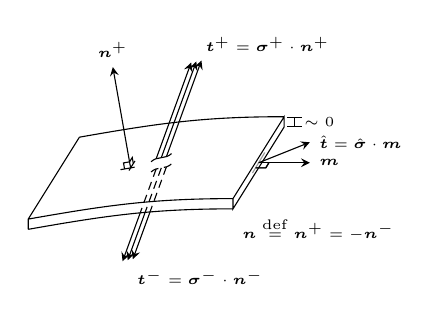
\begin{tikzpicture}[>=stealth,scale=1.3,font=\tiny]
 \coordinate (A) at (0,0);
 \coordinate (B) at (2,0.2);
 \coordinate (C) at (2.5,1);
 \coordinate (D) at (0.5,0.8);
 \coordinate (At) at (0,-0.1);
 \coordinate (Bt) at (2,0.1);
 \coordinate (Ct) at (2.5,0.9);

 \draw (A) to[out=10,in=180] (B)
      (At) to[out=10,in=180] (Bt)
      (Bt) -- (B) -- (C) coordinate[midway] (E) -- (Ct) -- cycle
      (At) -- (A) -- (D) to[out=10,in=180] (C);

 % Binormal m
 \draw[draw=black!40] (E)++(0,-0.05)++(-0.06,-0.1) -- +(0.12,0.2);
 \draw[->] (E)++(0,-0.05) -- +(0.5,0) node[right]{$\boldsymbol{m}$};
 \draw[->] (E)++(0,-0.05) -- +(0.5,0.2) node[right]{$\hat{\boldsymbol{t}}=\hat{\boldsymbol{\sigma}}\cdot\boldsymbol{m}$};
 \draw (E)++(-0.03,-0.1) -- ++(0.1,0) -- +(0.03,0.05);
 \draw (E)++(0,-0.05)++(-0.03,-0.05) -- ++(0.1,0) -- +(0.03,0.05);

 
 % Normal
 \coordinate (n) at (1,0.5);
 \draw[->] (n) -- +(100:1) node[above]{$\boldsymbol{n}^+$};
 \draw (n)++(190:0.06) -- ++(100:0.06) -- +(190:-0.06);
 \draw (n)++(190:0.1) -- +(190:-0.14);
 \draw (n)++(58:0.05) -- ++(100:0.06) -- +(58:-0.05);
 \draw (n)++(58:0.08) -- +(58:-0.11);
 %\draw (n)++(190:0.06) -- ++(58:0.05) -- ++(190:-0.06);
 
 % Traction +
 \draw[->] (1.3,0.6) -- +(70:1) node[above right]{$\boldsymbol{t}^+ = \boldsymbol{\sigma}^+\cdot\boldsymbol{n}^+$};
 \draw[->] (1.35,0.61) -- +(70:1);
 \draw[->] (1.25,0.59) -- +(70:1);
 \draw (1.2,0.56) to[out=45,in=-135] (1.4,0.64);

 % Traction -
 \draw[densely dashed] (1.3,0.5) -- +(-110:0.46) coordinate (tmin); \draw[->] (tmin) -- +(-110:0.5) node[below right]{$\boldsymbol{t}^- =  \boldsymbol{\sigma}^-\cdot\boldsymbol{n}^-$};
 \draw[densely dashed] (1.35,0.51) -- +(-110:0.46) coordinate (tmin); \draw[->] (tmin) -- +(-110:0.5);
 \draw[densely dashed] (1.25,0.49) -- +(-110:0.46) coordinate (tmin); \draw[->] (tmin) -- +(-110:0.5);
 \draw[densely dashed] (1.2,0.46) to[out=45,in=-135] (1.4,0.54);

 % Thickness
 \draw[|-|] ([xshift=0.1cm]C) -- ([xshift=0.1cm]Ct) node[midway,right] {$\sim 0$};

 % Definition
 \node[right] at (2,-0.1) {$\boldsymbol{n} \overset{\mathrm{def}}{=} \boldsymbol n^+ = -\boldsymbol n^-$};
\end{tikzpicture}}
 \end{center}
\vspace{-1em}
\begin{itemize}
 \item Equilibrium for tractions on smooth surface/interface segments
\vspace{-0.7em}
\begin{align*}
 \ta t^+ + \ta t^- + \ta t_\surf = \ta 0 \text{ on } \Gamma_i^{\mathrm{pore}} \text{ or } \Gamma_j^{\mathrm{cont}},\quad \ta t_\surf \defeq \hat{\ts\sigma}\cdot\hat{\ta\nabla}
\end{align*}
$\hat{\ts\sigma} =$ ``surface stress'' (in tangent plane), $\hat{\ta\nabla} =$ ``surface \rlap{gradient''}
 \item Particle/pore boundaries $\Gamma_i^{\mathrm{pore}}:\;\;\ta t\defeq \ts\sigma^-\cdot\ta n = \ta t_\surf$
\item Special case: Isotropic homogeneous surface tension: $\hat{\ts\sigma}=\gamma_\surf \hat{\ta I}$, $\hat{\ts I}\defeq\ts I-\ta n\outerp\ta n$ \vspace{-0.5em}
\begin{align*}
 \implies\quad \ta t_\surf = - \kappa \gamma_s \ta n,\quad \kappa \defeq \ta n \cdot \hat{\ta\nabla} \text{ (curvature)}
\end{align*}
 %\item \roughcite{Steinmann, Javili \& Steinmann (2009-)}
\end{itemize}
\end{frame}

%%%%%%%%%%%%%%%%%%%%%%%%%%%%%%%%%%%%%%%%%%%%%%%%%%%%%%%%%%%%%%%%%%%%%%%%%%%%%%%%%%%%%%%%%%%%%%%%%%%
% \begin{frame}
%  \frametitle{Surface tension on free surface and interfaces}
%  \begin{center}
%  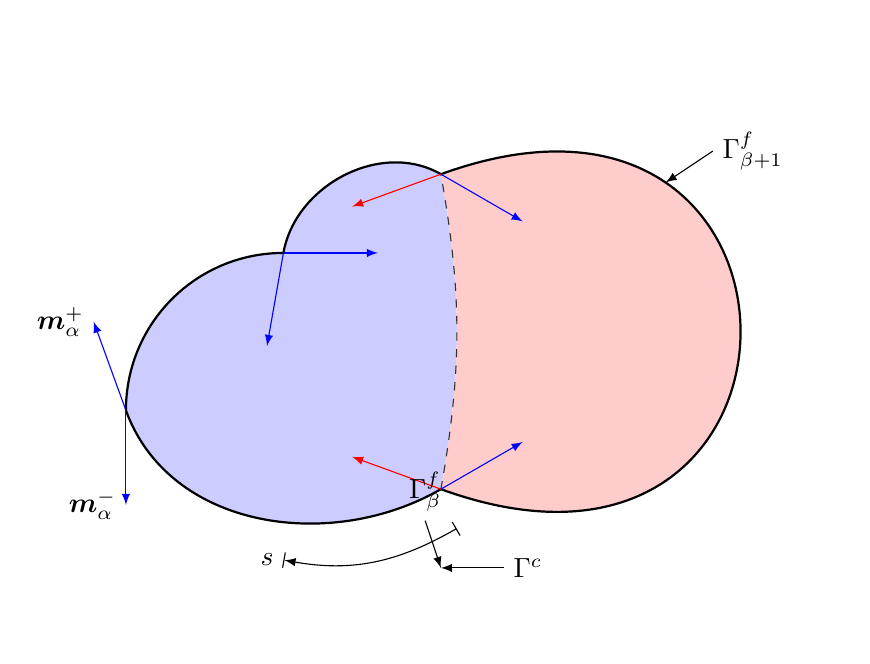
\begin{tikzpicture}[>=latex,scale=2]
  \def\mlength{0.6};
  % Fill
  \begin{scope}[red]
  	\clip (0,0.5) 
  		to[out=-150,in=-70] (-2,1)
  		to[out=90,in=180] (-1,2) 
  		to[out=80,in=150] (0,2.5)
  		to[out=-80,in=80] (0,0.5);
  	\fill[fill=blue!20] (-2,0) rectangle +(5,5);
  \end{scope}
  \begin{scope}
  	\clip (0,0.5) to[out=80,in=-80] (0,2.5) .. controls +(  20:2.7) and +(-20:2.7) .. (0,0.5);
  	\fill[fill=red!20] (-1,0) rectangle +(5,5);
  \end{scope}
  
  % Lines
  \draw[thick] (0,0.5) 
  		to[out=-150,in=-70] (-2,1)
  		to[out=90,in=180] (-1,2) 
  		to[out=80,in=150] (0,2.5) coordinate[midway] (GammaF1) 
  		.. controls +(20:2.7) and +(-20:2.7) .. (0,0.5) coordinate[near start] (GammaF2) -- cycle;
  \draw[dashed,black!80] (0,0.5) to [out=80,in=-80] (0,2.5) coordinate[midway] (GammaC);
  
  % Arrows
  \draw[->,red]  (0,0.5) -- +(180- 20:\mlength);
  \draw[->,blue] (0,0.5) -- +(180-150:\mlength);
  \draw[->,blue] (-2,1)  -- +(180- 70:\mlength) node[left,black] {$\text{\boldmath$m$}_\alpha^+$};
  \draw[->,blue] (-2,1)  -- +(180+ 90:\mlength) node[left,black] {$\text{\boldmath$m$}_\alpha^-$};
  \draw[->,blue] (-1,2)  -- +(180+180:\mlength);
  \draw[->,blue] (-1,2)  -- +(180+ 80:\mlength);
  \draw[->,blue] (0,2.5) -- +(180+150:\mlength);
  \draw[->,red]  (0,2.5) -- +(180+ 20:\mlength);
  
  % Annotations
  \draw[|->|] (0.1,0.25) to[out=-150,in=-10] (-1,0.05) node[left] {$s$};
  \draw[<-] (GammaC)  -- +( 0.4,0)   node[right] {$\Gamma^c$};
  \draw[<-] (GammaF1) -- +(-0.1,0.3) node[above] {$\Gamma_{\beta}^f$};
  \draw[<-] (GammaF2) -- +( 0.3,0.2) node[right] {$\Gamma_{\beta+1}^f$};
\end{tikzpicture}
%  \end{center}
% \vspace{-2em}
%  \begin{itemize}
%   \item Equilibrium for singular curve $C$ $\leadsto$ ``wetting'' angles
%   \begin{align*}
%    \sum_i \hat{\ta t}_i = \ta 0 \text{ on } C= \cap_i \Gamma_i, \quad \hat{\ts t}_i \defeq \hat{\ts\sigma}_i\cdot\ta m_i
%   \end{align*}
%  \end{itemize}
% \end{frame}

%%%%%%%%%%%%%%%%%%%%%%%%%%%%%%%%%%%%%%%%%%%%%%%%%%%%%%%%%%%%%%%%%%%%%%%%%%%%%%%%%%%%%%%%%%%%%%%%%%%
\begin{frame}
 \frametitle{Subscale constitutive modeling}
 \begin{itemize}
  \item Co-binder: Incompressible, viscous flow $\leadsto$ Stokes' flow.
  \begin{gather*}
   \ts\sigma_\dev = \mu^{\mathrm{Co}} {\ts d}_\dev\\
   \ts\sigma_\dev = \ts\sigma + p\ts I,\quad \ts d_\dev = [\ts v\outerp \diff]_\dev^\sym
  \end{gather*}
  \item WC-particles: ``Rigid'' $\to$ incompressible, approximated as Newtonian flow with ``large'' viscosity
  \begin{align*}
   \mu^{\mathrm{WC}} \gg \mu^{\mathrm{Co}}
  \end{align*}
  \item Quasistatic motion of viscoplastic particles, spatial setting:
  \begin{align*}
   -\ts\sigma(\ts d)\cdot\ta\nabla = \ta 0 \text{ in } \Omega^\particle,\quad \ta v\cdot\ta\nabla = 0 \text{ in } \Omega^\particle,\quad \Omega^\particle = \cup_\alpha \Omega_\alpha^\particle
  \end{align*}
  %\alert{Note}: Tangent ``stiffness'' $\tf E_{\mathrm{T},\dev}$ from $\dif\ts\sigma_\dev = \tf E_{\mathrm{T},\dev}\dprod \dif\ts d$ used in Newton iterations on subscale (RVE-problem)
 \end{itemize}
\end{frame}

\begin{frame}
 \frametitle{Weak form of ``fine-scale'' problem}
%\footnotesize
 \begin{itemize}
  \item Sintering particles occupying domain $\Omega^\particle$ with internal boundary $\Gamma^\pore \defeq (\cup_i \Gamma_i^\pore) \cup (\cup_j \Gamma_j^\contact)$:
Find $\ta v\in \set V, p\in \set P$

 such that
\begin{align*}
  \int_{\mathrlap{\Omega^\particle}} \;\ts\sigma\dprod[\delta\ta v\outerp\ta\nabla]\dif v &=
   \int_{\mathrlap{\Gamma^\pore}} \;\hat{\ts\sigma}\dprod[\delta\ta v\outerp\hat{\ta\nabla}] \dif a +
   \int_{\mathrlap{\Gamma_N^\external}} \;\ta t_p\cdot\delta\ta v\dif a \; && \forall \delta \ta v\in \set V^0 \\
  \int_{\mathrlap{\Omega^\particle}} \;[\ta v\cdot\ta\nabla]\delta p\dif v &= 0 && \forall \delta p\in \set P
\end{align*}
\alert{Note}: Obtained via use of surface divergence theorem + equilibrium for singular curves $C_i$

 \item \alert{Special case}: Isotropic surface tension (may be state-dependent and/or inhomogeneous along $\Gamma^\pore$)
 \begin{align*}
  \int_{\mathrlap{\Gamma^\pore}} \;\hat{\ts\sigma}\dprod[\delta\ta v\outerp\hat{\ta\nabla}] \dif a =
  \int_{\mathrlap{\Gamma^\pore}} \;\gamma_\surf[\delta\ta v\cdot\hat{\ta\nabla}] \dif a
 \end{align*}

 \end{itemize}

\end{frame}

\subsection{Homogenization}
%%%%%%%%%%%%%%%%%%%%%%%%%%%%%%%%%%%%%%%%%%%%%%%%%%%%%%%%%%%%%%%%%%%%%%%%%%%%%%%%%%%%%%%%%%%%%%%%%%%
\begin{frame}
 \frametitle{RVE-problem}
\begin{itemize}
 \item Homogenization on RVE occupying bulk volume $\Omega_\Box$ with external boundary $\Gamma_\Box$
 \begin{align*}
  \int_{\Omega^{\mathrm{part}}} f \dif v \stackrel{\text{replaced by}}{\to} \int_\Omega \langle f\rangle_\Box \dif \bar{v}, \quad \langle f\rangle_\Box \defeq \frac1{|\Omega_\Box|} \int_{\Omega_\Box^{\mathrm{part}}} f \dif v
 \end{align*}
 \item RVE in 2D with (circular) particles in a perfect square lattice \textcolor{blue}{(present state!)}. Contact surfaces are initially flattened from precompaction.
\end{itemize}
 \begin{center}
  \begin{columns}
   \column{0.2\textwidth}
   \column{0.3\textwidth}\centering
    \resizebox{!}{0.8\textwidth}{\begin{tikzpicture}[>=latex,scale=2] % Use this to scale the image. Text is always normal-size
  \def\particleradius{1.05} % Adjust this to change the contact size.
  \pgfmathsetmacro{\contactsize}{sqrt(\particleradius^2-1)} % Automatically calculated.
  \begin{scope}[very thick]
  	\draw[clip] (-1,-1) rectangle (1,1);
  	\draw[clip]
  		(-1,-1) circle (\particleradius)
 		( 1,-1) circle (\particleradius)
 		(-1, 1) circle (\particleradius)
   		( 1, 1) circle (\particleradius);
  	\fill[fill=black!10] (-1,-1) rectangle (1,1);
  \end{scope}
  % Markers
  \foreach \q in {0,90,180,270} { \draw[rotate=\q] (1-\contactsize,-0.05) -- +(0,0.1); }
  \draw[dashed,gray] (-1.1,0) -- (1.1,0) (0,-1.1) -- (0,1.1);
  % Annotations
  %\node[below] at (0,0) {$\Omega_\Box^p(0)$};
  \draw[|<->|] (-1,-1.4) -- (1,-1.4) node[midway,above] {$L_\Box(0)$};
  \draw[<->|] (-1,-0.05) -- +(\contactsize,0) node[midway,below] {$a_0$};
  \node at (0.6,-0.6) {$\Omega_\Box(0)$};
  \draw[<-] (1,-0.5) -- +(0.2,0) node[right] {$\Gamma_\Box(0)$};
  \draw[<-] (1,1) ++(-135:\particleradius) -- +(0.00,0.15) node[above right] {$\Gamma_\Box^{\mathrm{f}}(0)$};
  
  %\draw[use as bounding box] (-1.7,-1.5) rectangle (1.7,1.1);
  %\useasboundingbox (-1.7,-1.5) (1.7,1.1);
  % Transformation arrow (makes the picture very unaligned)
  %\draw[->] (1.5,0) to[out=45,in=-150] (2,0);% +(135:0.1) -- (2,0) -- +(-135:0.1);
\end{tikzpicture}
}
   %\column{0.3\textwidth}\centering
   % \resizebox{!}{0.8\textwidth}{\begin{tikzpicture}[>=latex,scale=1.8] % Use this to scale the image. Text is always normal-size
  \def\particleradius{1.05} % Adjust this to change the contact size.
  \draw[thick,fill=black!10,even odd rule] (0.9,-1.1) 
  	to[out=190,in=10] (-1.1,-0.9)
  	to[out=80,in=-110] (-0.9,1.1)
  	to[out=10,in=-160] (1.1,1.1)
  	to[out=-100,in=60] (0.9,-1.1) -- cycle
  	(-0.1,-0.5) to[out=180,in=-45] (-0.2,-0.15) to[out=135,in=-90]
  	(-0.5,0)    to[out=90,in=-135] (-0.15,0.15)  to[out=45,in=-180]  
  	(0.1,0.5)   to[out=0,in=135]   (0.2,0.15)   to[out=-45,in=90] coordinate[near start] (GammaF)
  	(0.5,0)     to[out=-90,in=45]  (0.15,-0.15)  to[out=-135,in=0] (-0.1,-0.5) -- cycle;
  % Markers
  \draw[dashed,gray] (-1.1,0) to[out=5,in=-175] (1.1,0) (-0.2,-1.1) -- (0.2,1.1);
  % Annotations
  \node at (0.5,-0.6) {$\Omega_\Box^{\mathrm{part}}(t)$};
  \draw[<-] (GammaF) -- +(0.00,0.15) node[above right] {$\Gamma_\Box^{\mathrm{pore}}(t)$};
\end{tikzpicture}}
   \column{0.2\textwidth}
  \end{columns}
 \end{center}
\end{frame}

%%%%%%%%%%%%%%%%%%%%%%%%%%%%%%%%%%%%%%%%%%%%%%%%%%%%%%%%%%%%%%%%%%%%%%%%%%%%%%%%%%%%%%%%%%%%%%%%%%%
% \begin{frame}
%  \frametitle{Homogenization of momentum balance}
%  \begin{itemize}
%     \item RVE-problem with Dirichlet b.c., ``driven'' by macroscale
%     rate-of-deformation $\bar{\ts d}\rightarrow$ subscale velocity:
%     $\ta{v}=\ta{v}^\macro(\bar{\ts d})+\ta{v}^\fluct$\\
%     For given $\bar{\ts d}$, solve for $\ta{v}^\fluct\in \set V_{\Box}^{\rm(D,0)}$, $p\in\set P_{\Box}$:
%    \vspace{-2.5truemm}
%  \end{itemize}
%     \begin{equation*}
% \begin{array}{rcll}
%     a_{\Box}(\ta{v}^\macro(\bar{\ts d})+\ta{v}^\fluct;\delta \ta{v}^\fluct) +  b_{\Box}(p,\delta\ta{v}^\fluct)
%     & = &
%     l_{\Box}(\delta \ta{v}^\fluct)
%     \quad & \forall \delta \ta{v}^\fluct\in\set V_{\Box}^{\rm (D,0)},
%     \\
%     b_{\Box}(\delta p,\ta{v}^\macro(\bar{\ts d})+\ta{v}^\fluct)
%     & = &
% %    - d_{\Box}(\delta \bi{t},\bbi{H}\cdot[\bi{X}-\bbi{X}])
%     0
%     \quad & \forall \delta p\in\set P_{\Box}.
% \end{array}
%     \end{equation*}
%    \vspace{-2.5truemm}
% %----------------------------------------------------------------------------
% \begin{align*}
%     a_\Box(\ta{v};\delta \ta{v})
%     & \defeq
%     \langle\ta{\sigma}_\dev(\ta{d}) : \delta \ta{d}\rangle_{\Box} =
%     \frac{1}{|\Omega_\Box|}\int_{\Omega^\particle_\Box} \ta{\sigma}_\dev(\ta{d}) \dprod \left[\delta \ta{v} \outerp \ta{\nabla}\right] \dif v
% \\
%     b_\Box(p, \ta{v})
%     & \defeq
%     - \langle p\ta{I} \dprod \ta{d}\rangle_{\Box} =
%     - \frac{1}{|\Omega_\Box|}\int_{\Omega^\particle_\Box} p\;\ta{v}\cdot \ta{\nabla} \dif v
% \\
%     l_\Box(\delta \ta{v})
%     & \defeq
%     \frac{1}{|\Omega_{\Box}|} \int_{\Gamma_{\Box}^\pore} \hat{\ts\sigma}\dprod\left[\delta\ta{v}\outerp\hat{\ts\nabla}\right] \dif a =
%     \frac{1}{|\Omega_{\Box}|} \int_{\Gamma_{\Box}^\pore}
% 	\gamma_\surf\left[\delta\ta{v}\cdot\hat{\ta\nabla}\right] \dif a
% \end{align*}
% %----------------------------------------------------------------------------
% \vspace{-2.5truemm}
%     $l_{\Box}(\delta \ta{v}^\fluct)$: loading by surface tension tractions on ${\Gamma}^\pore_{\Box}$
% \end{frame}

%%%%%%%%%%%%%%%%%%%%%%%%%%%%%%%%%%%%%%%%%%%%%%%%%%%%%%%%%%%%%%%%%%%%%%%%%%%%%%%%%%%%%%%%%%%%%%%%%%%
% \begin{frame}
%  \frametitle{Macroscale problem}
%  \begin{itemize}
% 
%     \item Macroscale momentum balance for ``free sintering'' (no external loading) obtained from variationally consistent homogenization
%     \vspace{-1em}
%     \begin{align*}
%    \bar{a}\{\bar{\ta v}; \delta \bar{\ta v}\} \defeq
%     \int_{\Omega} \bar{\ts \sigma}\{\bar{\ts d}\} \dprod \delta \bar{\ts d}
%     \dif\bar{v} = 0
%     \end{align*}
%     Macroscale stress:
%     \vspace{-2.5truemm}
%     \begin{align*}
%     \bar{\ts\sigma}=\frac{1}{|\Omega_{\Box}|}\int_{\Gamma_{\Box}}
%     \ta{t}\outerp[\ta{x}-\bar{\ta x}] \dif a, \,\,\bar{\ta x}= \mbox{ center of RVE}
%     \end{align*}
%     \textbf{Note}: Variational format valid only for macroscale compressibility (before porosity has vanished locally)
% 
%     \item Algorithmic features for macroscale problem
%     \begin{itemize}
%         \item[-] Linear $\bar{\ta v}$
%         \item[-] Explicit time-stepping
%         \item[-] ATS-tensor obtained from sensitivity analysis of RVE-problem.
%         \item[-] Parallel processing,  almost linear scaling of CPU-time with no. of processors due to parallelization at macroscale quadrature points
%     \end{itemize}
% \end{itemize}
% \end{frame}

%%%%%%%%%%%%%%%%%%%%%%%%%%%%%%%%%%%%%%%%%%%%%%%%%%%%%%%%%%%%%%%%%%%%%%%%%%%%%%%%%%%%%%%%%%%%%%%%%%%
\begin{frame}
 \frametitle{FE\textsuperscript{2} format: Standard (velocity-based) macroscale equation}
 \begin{itemize}
  \item Validity is restricted to macroscopically compressible response ($\bar{e} \defeq \bar{\ts d} \dprod \ts I = \bar{\ta v}\cdot \diff\neq 0$)
 \end{itemize}
 \begin{itemize}
  \item Macroscale-problem
  \begin{itemize}
   \item Fields: $\bar{\ta v}$%, solved from \eqref{eq:macro_problem_old}
  \end{itemize}
  \item RVE-problem: $\bar{\ts d}_\dev, \bar{e} \longrightarrow \bar{\ts\sigma}_\dev, \bar{p}$
  \begin{itemize}
   \item Input: $\bar{\ts d}$ (or $\bar{\ts d}_\dev, \bar{e}$)
   \item Fields: $\ta v^\fluct$, $p$%, solved from \eqref{eq:rve_problem_old}
   \item Output: $\bar{\ts\sigma}$ (or $\longrightarrow \bar{\ts\sigma}_\dev, \bar{p}$) (post-processed)
  \end{itemize}
 \end{itemize}

 \begin{itemize}
   \item \roughcite{\"Ohman et al. (2012) Tech. Mechanik}
 \end{itemize}

%  \begin{itemize}
%   \item[-] No free surfaces (zero porosity) $\leadsto$ Unknown subscale pressure field; singular tangent, $\ts I\dprod \bar{\tf E}\dprod \ts I\to \infty$
%   \item[-] Requires new macroscopic formulation
%  \end{itemize}

\end{frame}

%%%%%%%%%%%%%%%%%%%%%%%%%%%%%%%%%%%%%%%%%%%%%%%%%%%%%%%%%%%%%%%%%%%%%%%%%%%%%%%%%%%%%%%%%%%%%%%%%%%
\begin{frame}
 \frametitle{FE\textsuperscript{2} format: Mixed macroscale equation}
 \begin{itemize}
  \item Introduce macroscale pressure $\bar{p}$ as independent variable, impose identity $\bar{e} = \bar{\ta v}\cdot \diff$ in a weak sense
 \end{itemize}

 \begin{itemize}
  \item Macroscale-problem (mixed format)
  \begin{itemize}
   \item Fields: $\bar{\ta v}$, $\bar{p}$%, solved from  \eqref{eq:new_macro}
  \end{itemize}
  \item RVE-problem: $\bar{\ts d}_\dev, \bar{p} \longrightarrow \bar{\ts\sigma}_\dev, \bar{e}$
  \begin{itemize}
   \item Input: $\bar{\ts d}_\dev$, $\bar{p}$
   \item Fields: $\ta v^\fluct$, $p$, $\bar{e}$%, solved from \eqref{eq:rve_problem_new}
   \item Output: $\bar{\ts\sigma}_\dev$ (post-processed), $\bar{e}$
  \end{itemize}
 \end{itemize}

 \begin{itemize}
  \item Valid for seamless transition from compressible to incompressible macroscale response.
 \end{itemize}
\end{frame}

%%%%%%%%%%%%%%%%%%%%%%%%%%%%%%%%%%%%%%%%%%%%%%%%%%%%%%%%%%%%%%%%%%%%%%%%%%%%%%%%%%%%%%%%%%%%%%%%%%%
% \subsection{Results}
% \begin{frame}
%  \frametitle{Numerical results: Single RVE - Macroscopically rigid}
% \vspace{-0.8em}
% \begin{figure}[thpb!]
%     \centering
%     \includegraphics[scale=0.1]{figures/evolve_fixed_a}
% %    \subfloat[$t = 0$]{\includegraphics[width=0.2\linewidth]{figures/evolve_fixed_3x3_a}\label{fig:evolve_fixed_a}}
%     \hspace{0.5em}
%     \includegraphics[scale=0.1]{figures/evolve_fixed_b}
% %    \subfloat[$t = \frac12 t_{\mathrm{end}}$]{\includegraphics[width=0.2\linewidth]{figures/evolve_fixed_3x3_b}\label{fig:evolve_fixed_b}}
%     \hspace{0.5em}
%     \includegraphics[scale=0.1]{figures/evolve_fixed_c}
% %    \subfloat[$t = t_{\mathrm{end}}$]{\includegraphics[width=0.2\linewidth]{figures/evolve_fixed_3x3_c}\label{fig:evolve_fixed_c}}
%     \hspace{0.5em}
%     \includegraphics[scale=0.1]{figures/evolve_fixed_d}
%     \caption{Snapshots of computed RVE-configurations at selected times. Fixed boundaries $\Gamma_\Box$: $\bar{\ts d}= \ts 0$}
%     \label{fig:fixed}
%     \vspace{-0.5em}
%   \begin{tikzpicture}
%   \begin{axis}[ xtick={0,0.2,...,1},
%                 tick label style={font=\scriptsize},font=\footnotesize,
%                 legend style={ at={(1.03,0.5)}, anchor=west },
%                 height=0.3\textwidth, width=0.7\textwidth, xmin=0, xmax=1, ymax=0,
%                 xlabel={$t/t_{\mathrm{end}}$}, ylabel={$\bar\sigma_\mean/p_\nominal$}]
%     \addplot[thick] file {figures/s_mean_fixed_1.txt}; \addlegendentry{$1\times1$}
%     \addplot[thick,red,densely dashed] file {figures/s_mean_fixed_3.txt}; \addlegendentry{$3\times3$}
%     \addplot[thick,blue,densely dotted] file {figures/s_mean_fixed_5.txt}; \addlegendentry{$5\times5$}'
%   \end{axis}
%   \end{tikzpicture}
% \end{figure}
% \vspace{-1em}
% \alert{Note}: Periodic b.c. gives independence of RVE-size for present assumption of oversimplified periodic microstructure!
% \end{frame}

%%%%%%%%%%%%%%%%%%%%%%%%%%%%%%%%%%%%%%%%%%%%%%%%%%%%%%%%%%%%%%%%%%%%%%%%%%%%%%%%%%%%%%%%%%%%%%%%%%%
% \begin{frame}
%  \frametitle{Numerical results: Single RVE - Macroscopically isochoric}
%  \vspace{-0.8em}
% \begin{figure}[thpb!]
%     \centering
%     \includegraphics[scale=0.1]{figures/evolve_shear_a}
%     %\subfloat[$t = 0$]{\includegraphics[scale=0.2]{figures/evolve_shear_1}\label{fig:evolve_shear_a}}
%     \hspace{0.5em}
%     \includegraphics[scale=0.1]{figures/evolve_shear_b}
%     %\subfloat[$t = \frac12 t_{\mathrm{end}}$]{\includegraphics[scale=0.2]{figures/evolve_shear_250}\label{fig:evolve_shear_b}}
%     \hspace{0.5em}
%     \includegraphics[scale=0.1]{figures/evolve_shear_c}
%     %\subfloat[$t = t_{\mathrm{end}}$]{\includegraphics[scale=0.2]{figures/evolve_shear_500}\label{fig:evolve_shear_c}}
%     \hspace{0.5em}
%     \includegraphics[scale=0.1]{figures/evolve_shear_d}
%     \caption{Snapshots of computed RVE-configurations at selected times. Constant shear rate on $\Gamma_\Box$: $\bar{\ts d}= \bar d_{12}(\bee 12 + \bee 21)$}
%     \label{fig:constant_shear}
%     \vspace{-0.5em}
%   \begin{tikzpicture}
%   \begin{axis}[ xtick={0,0.2,...,1},
%                 tick label style={font=\scriptsize},font=\footnotesize,
%                 legend style={ at={(1.03,0.5)}, anchor=west },
%                 height=0.3\textwidth, width=0.7\textwidth, xmin=0, xmax=1,ymax=0,
%                 xlabel={$t/t_{\mathrm{end}}$}, ylabel={$\bar\sigma_\mean/p_\nominal$}]
%     \addplot[thick] file {figures/s_mean_shear_1.txt}; \addlegendentry{$1\times1$}
%     \addplot[thick,red,densely dashed] file {figures/s_mean_shear_3.txt}; \addlegendentry{$3\times3$}
%     \addplot[thick,blue,densely dotted] file {figures/s_mean_shear_5.txt}; \addlegendentry{$5\times5$}
%   \end{axis}
%   \end{tikzpicture}
% \end{figure}
% \vspace{-1em}
% \alert{Note}: Periodic b.c. gives independence of RVE-size for present assumption of oversimplified periodic microstructure!
% \end{frame}

%%%%%%%%%%%%%%%%%%%%%%%%%%%%%%%%%%%%%%%%%%%%%%%%%%%%%%%%%%%%%%%%%%%%%%%%%%%%%%%%%%%%%%%%%%%%%%%%%%%
% \begin{frame}
%  \frametitle{Numerical results: Single RVE -- Free sintering}
% \begin{center}
%  \vspace{-1em}
% \begin{itemize}
%  \item \movie[externalviewer]{Condition of free sintering: $\bar{\ts\sigma} = \ts 0$}{free_3x3.wmv}
%  \item Evolution of porosity $\Phi \defeq |\Omega_\Box^{\mathrm{pore}}|/|\Omega_\Box|$
% \end{itemize}
% \movie[height=4cm,width=4cm,poster]{\includegraphics[width=4cm]{figures/free_1x1.0000}}{free_1x1.wmv}
% \movie[height=4cm,width=4cm,poster]{\includegraphics[width=4cm]{figures/free_3x3.0000}}{free_3x3.wmv}
%   \begin{tikzpicture}
%   \begin{axis}[ yticklabel style={ /pgf/number format/fixed, /pgf/number format/precision=2 },
%                 tick label style={font=\tiny},font=\footnotesize,
%                 height=0.4\textheight, width=0.9\textwidth, xmin=0, xmax=1400, ymin=0.83,
%                 legend style={font=\tiny,at={(1,0)},anchor=south east},
%                 xlabel={Time step}, ylabel={$1-\Phi$}]
%     \addplot[thick,black] file {figures/porosity_1x1.txt}; \addlegendentry{$1\times1$}
%     \addplot[thick,red,densely dashed] file {figures/porosity_3x3.txt}; \addlegendentry{$3\times3$}
%     \addplot[thick,blue,densely dotted] file {figures/porosity_5x5.txt}; \addlegendentry{$5\times5$}
%   \end{axis}
%   \end{tikzpicture}
% \end{center}
% \end{frame}

%%%%%%%%%%%%%%%%%%%%%%%%%%%%%%%%%%%%%%%%%%%%%%%%%%%%%%%%%%%%%%%%%%%%%%%%%%%%%%%%%%%%%%%%%%%%%%%%%%%
% \subsection{Remeshing strategies}
% \begin{frame}
%  \frametitle{Surface tracking}
%  \vspace{-1em}
%  \begin{columns}
% \column{0.5\textwidth}
%  \begin{figure}[!ht]
%  \centering
%  \includegraphics[width=0.9\textwidth]{figures/gbpm_example}
%  \caption{Part of the mesh with its boundary tracking particles}\label{fig:examples_particles}
% \end{figure}
% \column{0.5\textwidth}
% \begin{figure}[!ht]
%  \centering
%  \scalebox{0.67}{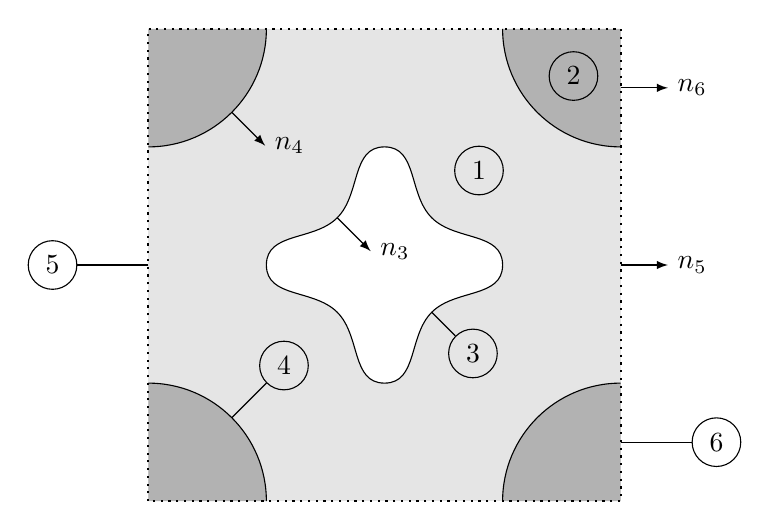
\begin{tikzpicture}[scale=3]
  \fill[black!10] (-1,-1) rectangle (1,1);
  \fill[fill=black!30]
   (-1,-1) -- ++(0.5,0)  arc (0:90:0.5) -- cycle
   ( 1,-1) -- ++(-0.5,0) arc (180:90:0.5) -- cycle
   ( 1, 1) -- ++(-0.5,0) arc (180:270:0.5) -- cycle
   (-1, 1) -- ++(0.5,0) arc (0:-90:0.5) -- cycle;
  \draw[draw=black, thick, dotted] (-1,-1) rectangle (1,1);
  \draw[black]
   (-1,-1)  ++(0.5,0)  arc (0:90:0.5)
   ( 1,-1)  ++(-0.5,0) arc (180:90:0.5)
   ( 1, 1)  ++(-0.5,0) arc (180:270:0.5)
   (-1, 1)  ++(0.5,0) arc (0:-90:0.5);
  \filldraw[fill=white, draw=black]
   (0,-0.5) to[out=180,in=-45] (-0.2,-0.2) to[out=135,in=-90]
   (-0.5,0) to[out= 90,in=-135](-0.2,0.2)  to[out=45,in=-180]
   (0,0.5)  to[out=  0,in=135] (0.2,0.2)   to[out=-45,in=90] 
   (0.5,0)  to[out=-90,in=45]  (0.2,-0.2)  to[out=-135,in=0] coordinate[at start] (boundary3) (0,-0.5) -- cycle;

 % Normals
 \draw[-latex] (-0.64645,0.64645) -- +(-45:0.2) node[right]{$\ta n_4$};
 \draw[-latex] (-0.2,0.2) -- +(-45:0.2) node[right]{$\ta n_3$};
 \draw[-latex] (1,0.75) -- +(0:0.2) node[right]{$\ta n_6$};
 \draw[-latex] (1,0) -- +(0:0.2) node[right]{$\ta n_5$};

 \node[draw,circle] at (0.4,0.4) {$1$};
 \node[draw,circle] at (0.8,0.8) {$2$};
 \draw[-] (boundary3) -- +(0.1,-0.1) node[draw,circle,at end,below right] at (0.8,0.8) {$3$};
 \draw[-] (-0.64645,-0.64645) -- (-0.5,-0.5) node[draw,circle,at end,above right] at (0.8,0.8) {$4$};
 \draw[-] (-1,0) -- +(-0.3,0) node[draw,circle,at end,left] at (0.8,0.8) {$5$};
 \draw[-] (1,-0.75) -- + (0.3,0) node[draw,circle,at end,right] at (0.8,0.8) {$6$};
 \end{tikzpicture}}\vskip -0.5em
%  \caption{Possible boundaries and regions required by the topology description}\label{fig:topology_boundaries}
% \end{figure}
% \end{columns}
%  \begin{itemize}
%   \item Implicit description of regions based on particles with normals.
%   \item Enumeration of all possible surfaces, including boundary conditions.
%   \item \roughcite{Leung \& Zhao (2009)}
%  \end{itemize}
% \end{frame}

%%%%%%%%%%%%%%%%%%%%%%%%%%%%%%%%%%%%%%%%%%%%%%%%%%%%%%%%%%%%%%%%%%%%%%%%%%%%%%%%%%%%%%%%%%%%%%%%%%%
% \begin{frame}
%  \frametitle{Remeshing}
%  \begin{figure}[!ht]
%  \centering
%  \includegraphics[width=0.4\textwidth]{figures/mesh_0}
%  \includegraphics[width=0.4\textwidth]{figures/mesh_1}
% \end{figure}
%  \begin{itemize}
%   \item Complete remeshing from surface description based on mesh deformation criterion.
%   \item Necessary coarsening (singularity at vanishing pores).
%   \item \alert{Note}: Noticeable source of discretization error.
%  \end{itemize}
% \end{frame}

%%%%%%%%%%%%%%%%%%%%%%%%%%%%%%%%%%%%%%%%%%%%%%%%%%%%%%%%%%%%%%%%%%%%%%%%%%%%%%%%%%%%%%%%%%%%%%%%%%%
% \subsection{Macroscale}
% \begin{frame}
%  \frametitle{Numerical results FE\textsuperscript{2}}
% \begin{columns}
% \column{0.5\textwidth}
% %  Subscale
% %  \begin{itemize}
% %   \item $a_\Box(\ta v^{\mathrm{M}}(\bar{\ta d})+\ta v^{\mathrm{s}};\delta v^{\mathrm{s}}) + \mathrlap{b_\Box(p,\delta\ta v^{\mathrm{s}}) = l_\Box(\delta\ta v^{\mathrm{s}})}$
% %   \item $ b_\Box(\delta p, \ta v^{\mathrm{M}}(\bar{\ta d}+\ta v^{\mathrm{s}}) = 0 $
% %   \item Dirichlet b.c. on RVE
% %   \item Very large deformations $\implies$ Remeshing.
% %  \end{itemize}
% %
% %  Macroscale
% %  \begin{itemize}
% %   \item $\bar a(\bar{\ta v},\delta\bar{\ta v}) = 0$
% %   \item Momentum balance with internal volumetric stress.
% %   \item \alert{Present limitation:} When pores vanish, RVE's become incompressible.
% %  \end{itemize}
% 
%  \begin{itemize}
%   \item FE\textsuperscript{2} of sintering of unloaded component at fixed temperature (constant material parameters).
%   \item Non-homogeneous $\rho_0'$, truly unrestrained macro--boundaries $\leadsto$ macroscale distortion (sheared RVE's).
%  \end{itemize}
% 
% \column{0.49\textwidth}
% 
% % \begin{center}
% %  \includegraphics[width=0.9\linewidth]{figures/macro_sintering_2x2.0000}\\
% %  $\longrightarrow$\\[0.5em]
% %  \includegraphics[width=0.9\linewidth]{figures/macro_sintering_2x2.0176}
% % \end{center}
% \end{columns}
% 
% \end{frame}

%%%%%%%%%%%%%%%%%%%%%%%%%%%%%%%%%%%%%%%%%%%%%%%%%%%%%%%%%%%%%%%%%%%%%%%%%%%%%%%%%%%%%%%%%%%%%%%%%%%
% \subsection{Results}
% \begin{frame}
%  \frametitle{Numerical results FE\textsuperscript{2}}
% \begin{center}
% \movie[width=\linewidth]{\includegraphics[width=\linewidth]{figures/macro_sintering_2x2.0000}}{macro_sintering_2x2.wmv}
% %1120x394 movie
% \movie[externalviewer]{FE\textsuperscript{2}-inhomogeneous component}{Sintering_5x5.mpeg}
% \end{center}
% \end{frame}

%%%%%%%%%%%%%%%%%%%%%%%%%%%%%%%%%%%%%%%%%%%%%%%%%%%%%%%%%%%%%%%%%%%%%%%%%%%%%%%%%%%%%%%%%%%%%%%%%%%
% \section{Paper B}
% \begin{frame}
%  \frametitle{Paper B:\\FE\textsuperscript{2} for Liquid-Phase Sintering with Seamless Transition from Macroscopic Compressibility to Incompressibility}
%  \begin{itemize}
%   \item Macroscale problem in Paper A breaks down for $\Phi = 1-\rho' = 0$.
%   \item Remedy: Mixed macroscale formulation
%   \item Dirichlet boundary conditions for mixed control in $\bar{\ts d}_\dev$ and $\bar p$
%   \item Numerical example of single RVE
%  \end{itemize}
% \end{frame}

% \subsection{Original problem}
% \begin{frame}
%  \frametitle{Macroscopically incompressible RVE's}
%  \begin{itemize}
%   \item Subscale features
%  \begin{itemize}
%   \item[-] No free surfaces $\leadsto$ Unknown subscale pressure field.
%   \item[-] Could be dealt with by prescribing pressure
%  \end{itemize}
% 
%  \item Macroscopic features
%  \begin{itemize}
%   \item[-] Singular tangent, $\ts I\dprod\bar{\tf E}\dprod\ts I\to\infty$
%   \item[-] Requires new macroscopic formulation
%  \end{itemize}
%  \end{itemize}
% 
% \end{frame}

%%%%%%%%%%%%%%%%%%%%%%%%%%%%%%%%%%%%%%%%%%%%%%%%%%%%%%%%%%%%%%%%%%%%%%%%%%%%%%%%%%%%%%%%%%%%%%%%%%%
\subsection{Macroscale}
\begin{frame}
 \frametitle{Macroscale problem}
\begin{itemize}
 \item Macroscale equations representing momentum balance and weak format of $\bar{e} = \bar{\ta v}\cdot\diff$
 \item Macroscale pressure $\bar{p}$ is a Lagrange multiplier
 \item Solve for $(\bar{\ta v}, \bar{p}) \in \bar{\set{V}}\times\bar{\set{P}}$ that solve the system
\end{itemize}

\begin{alignat*}{3}
 &\int_\Omega \bar{\ts\sigma}_\dev\{\bar{\ts d}_\dev,\bar{p}\} \dprod [\delta\bar{\ta v}\outerp \diff] \dif v + \int_\Omega -\bar{p}\;[\delta\bar{\ta v}\cdot\diff]\dif v &&= 0 &\quad& \forall \delta\bar{\ta v}\in \bar{\set{V}}^0\\
 &\int_\Omega \left[\bar{e}\{\bar{\ts d}_\dev,\bar{p}\} - \bar{\ta v}\cdot\diff\right]\delta\bar{p} \dif v &&= 0&\quad& \forall \delta\bar{p}\in \bar{\set{P}}
\end{alignat*}

\begin{align*}
 \bar{\ts\sigma}_\dev = \frac{1}{|\Omega_\Box|} \int_{\Gamma_\Box} \ta t \outerp [\ta x - \bar{\ta x}]\dif v + \bar{p}\ts I
\end{align*}

%     \begin{align*}
%  \bar a\{\bar{\ta v},{\color{red}\bar p}; \delta\bar{\ta v}\} + \bar b\{\bar p, \delta\bar{\ta v}\} &= \bar l\{\delta\bar{\ta v}\}   &&\quad \forall\; \delta\bar{\ta v} \in \bar{\set{V}}^0
%  \\
%  \bar b\{\delta\bar p, \bar{\ta v}\} + {\color{red}\bar c\{\bar{\ta v}, \bar p; \delta\bar p\}}&= 0   &&\quad \forall\; \delta\bar p \in \bar{\set{P}}
%      \end{align*}
% 
% \begin{align*}
%  \bar a\{\bar{\ta v},{\color{red}\bar p}; \delta\bar{\ta v}\} &\defeq \int_\Omega \bar{\ts\sigma}_{\Box,\dev}\{\left[\bar{\ta v}\outerp \diff\right]^\sym_\dev,{\color{red}\bar p}\}\dprod \left[\delta\bar{\ta v}\outerp \diff\right]^\sym_\dev \dif v
%  \\
%  \bar b\{\bar p, \delta\bar{\ta v}\}             &\defeq -\int_\Omega \bar p\left[\delta\bar{\ta v}\cdot\diff\right]\dif v
%  \\
%  \color{red}\bar c\{\bar{\ta v}, \bar p; \delta\bar p\}     &\color{red}\defeq \int_\Omega \bar d_{\Box,\vol}\{\left[\bar{\ta v}\outerp \diff\right]^\sym_\dev,\bar p\}\delta\bar p\dif v
%  \\
%  \bar l\{\delta\bar {\ta v}\}               &\defeq \int_{\Gamma^\external_\Neumann} \bar{\ta t}_\prescribed\cdot \delta\bar{\ta v} \dif a
% \end{align*}
\end{frame}


% \begin{frame}
%  \frametitle{New macroscale problem}
%  \begin{itemize}
%     \item Additional tangents
% \begin{align*}
%  \dif \bar{\ts\sigma}_{\Box,\dev} &= {\color{red}\bar{\tf E}_\ded} \dprod \dif\bar{\ts d}_\dev + {\color{red}\bar{\ts E}_\dep} \dif\bar{p}
%  \\
%  \dif \bar{d}_{\Box,\vol} &= {\color{red}\bar{\ts C}_\ded} \dprod \dif \bar{\ts d}_\dev + {\color{red}\bar{C}_\dep} \dif\bar{p}
% \end{align*}
%  \item \alert{Note}: $\bar{\ts E}_\dep = \bar{\ts C}_\ded$ and $\bar{\tf E}_\ded = \bar{\tf E}_\ded^\sym$ if the RVE-problem can be represented by the minimization of a potential.
%  \end{itemize}
% \end{frame}

% \subsection{RVE-problem}
% \begin{frame}
%  \frametitle{RVE-problem for mixed control}
%  \begin{itemize}
%   \item Prescribed $\bar{\ts d}_\dev$ and $\bar p$ instead of $\bar{\ts d}$, i.e:
% \end{itemize}
%   \begin{align*}
%    \bar{\ts\sigma}_{\dev}=\bar{\ts\sigma}_{\Box,\dev}\{\bar{\ts d}_\dev,\bar p\},\quad \bar{d}_{\vol} = \bar{d}_{\Box,\vol}\{\bar{\ts d}_\dev,\bar p\}
%   \end{align*}
% \begin{itemize}
%  \item Weak format of equilibrium for an RVE
% \end{itemize}
% \begin{align*}
%     \underbrace{\frac{1}{|\Omega_\Box|}\int_{\Omega^\particle_\Box} \ts{\sigma}([\ta v\outerp\diff]^\sym) \dprod \left[\delta \ta{v}\outerp\diff\right]^\sym \dif v}_{a_\Box(\ta v;\delta\ta v) + b_\Box(p,\delta\ta v)} =
%     \underbrace{\frac{1}{|\Omega_\Box|}\int_{\Gamma_\Box\cup\Gamma_\Box^\pore} \ta{t} \cdot \delta\ta{v} \dif a}_{l_\Box(\delta\ta v)+l_\Box^\pore(\delta\ta v)}
% \end{align*}
% \begin{itemize}
%   \item Introducing the split in velocity, using first order homogenization;
%  \end{itemize}
%   \begin{align*}
%    \ts v = \ts v^\macro + \ts v^\fluct = \bar{\ts d}\cdot[\ta x - \bar{\ta x}] + \ta v^\fluct = 
%     \underbrace{\bar{\ts d}_\dev\cdot[\ta x-\bar{\ta x}]}_{\ta v^\macro_\dev}+\bar d_\vol\underbrace{\frac13[\ta x-\bar{\ta x}]}_{\ta x_\mean} + \ta v^\fluct
%   \end{align*}
% \end{frame}

% \begin{frame}
%  \frametitle{RVE-problem:}
%  \begin{itemize}
%   \item Test the weak format of equilibrium with $\delta\ta v^\fluct \in \set V_\Box^{(\Dirichlet)}$ (trivial):
% \end{itemize}
%   \begin{align*}
%    a_\Box(\ta v; \delta\ta v^\fluct) + b_\Box(p,\delta\ta v^\fluct) = l_\Box^\pore(\delta\ta v^\fluct)
%   \end{align*}
% \begin{itemize}
%  \item Testing with $\delta\ta v^\macro_\vol = \delta\bar d_\vol \ta x_\mean$
% \end{itemize}
% \begin{gather*}
%     - \left[\frac{1}{|\Omega_\Box|}\int_{\Omega^\particle_\Box} p  \dif v \right]\delta\bar{d}_\vol =
%     \left[\frac{1}{|\Omega_\Box|}\int_{\Gamma_\Box^\pore} \ta{t}_\surf \cdot \ta{x}_\mean \dif a
%     - \bar{p}\right]\delta\bar{d}_\vol\\
%     \Longleftrightarrow\\
% b_\Box(p,\delta\ta v) = [l_\Box^\pore(\ta x_\mean) - \bar p]\delta\bar d_\vol
% \end{gather*}
% \end{frame}

\begin{frame}
\frametitle{RVE-problem for mixed control: Dirichlet b.c.}
 \begin{itemize}
  \item For given macroscale variables $\bar{\ts d}_\dev$ and $\bar p$, find ($\bar{e},p,\ta{v}^\fluct)\in\set{R}\times\set{V}_\Box^{(\Dirichlet)}\times\set{P}_\Box$ that solve the system
 \end{itemize}
\vspace{-2truemm}
\begin{alignat*}{4}
    & a_\Box(\ta{v}^\macro_\dev + \ta{v}^\fluct;\delta \ta{v}^\fluct) +  b_\Box(p,\delta\ta{v}^\fluct)
    && =
    l^\pore_\Box(\delta \ta{v}^\fluct)
    &\quad& \forall\; \delta \ta{v}^\fluct &&\in \set{V}_\Box^{(\Dirichlet)}
 \\
    &b_\Box(\delta p, \bar{e} \ta x_\mean +\ta{v}^\fluct)
    && =
    0
    && \forall\; \delta p &&\in \set{P}_\Box
\\
    &b_\Box(p,\ta{x}_\mean)\delta\bar{e}
    && =
    [l_\Box^\pore(\ta{x}_\mean) - \bar{p}]\delta\bar{e}
    && \forall\; \delta\bar{e} &&\in \set{R}
\end{alignat*}
\vspace{-5truemm}
\begin{align*}
    a_\Box(\ta{v};\delta \ta{v})
    & \defeq
    %\langle\ta{\sigma}_\dev(\ta{d}) : \delta \ta{d}\rangle_{\Box} =
    \frac{1}{|\Omega_\Box|}\int_{\Omega^\particle_\Box} \ta{\sigma}_\dev(\ta{d}) \dprod \left[\delta \ta{v} \outerp \diff\right] \dif v
\\
    b_\Box(p, \ta{v})
    & \defeq
    %\langle -p\ta{I} \dprod \ta{d}\rangle_{\Box} =
    \frac{1}{|\Omega_\Box|}\int_{\Omega^\particle_\Box} -p\;[\ta{v}\cdot \diff] \dif v
\\
    l_\Box(\delta \ta{v})
    & \defeq
    %\frac{1}{|\Omega_{\Box}|} \int_{\Gamma_{\Box}^\pore} \hat{\ts\sigma}\dprod\left[\delta\ta{v}\outerp\hat{\diff}\right] \dif a =
    \frac{1}{|\Omega_{\Box}|} \int_{\Gamma_{\Box}^\pore}
  \gamma_\surf\left[\delta\ta{v}\cdot\hat{\ta\nabla}\right] \dif a
\end{align*}
\begin{gather*}
 \ta v_\dev^\macro \defeq \bar{\ts d}_\dev \cdot[\ta x - \bar{\ta x}],\quad \ta{x}_\mean \defeq \frac13[\ta x-\bar{\ta x}], \quad \bar{\ta x} = \text{RVE center}
\end{gather*}
% \begin{itemize}
%  \item \alert{Note}: Still a Dirichlet boundary condition; $\ta v^\fluct = \ta 0$ on $\Gamma_\Box$.
% \end{itemize}
\end{frame}


% \begin{frame}
% \frametitle{RVE-problem sensitivity analysis}
%  \begin{itemize}
%   \item Perturbations $\bar{\ts d}_\dev + \dif\bar{\ts d}_\dev$ and $\bar p + \dif \bar p$ in the linearized problem
%  \end{itemize}
% \begin{alignat*}{4}
%     &(a_\Box)'(\bullet;\delta\ta{v}^\fluct,\dif\ta{v}^\macro_\dev + \dif\ta{v}^\fluct) +
%     b_\Box(\dif p,\delta\ta{v}^\fluct)
%     && = 0
%     &\quad& \forall\; \delta \ta{v}^\fluct &&\in \set{V}_\Box^{(\Dirichlet)}
%  \\
%     &b_\Box(\delta p,\dif\ta{v}^\macro_\vol + \dif\ta{v}^\fluct)
%     && = 0
%     && \forall\; \delta p &&\in \set{P}_\Box
% \\
%     &b_\Box(\dif p,\ta{x}_\mean)\delta\bar{d}_\vol
%     && = -\dif\bar{p}\delta\bar{d}_\vol
%     && \forall\; \delta\bar{d}_\vol &&\in \set{R}
% \end{alignat*}
% \begin{itemize}
%  \item Sensitivity fields used to obtain the tangents; $\tf E_\ded$, $\ts E_\dep$, $\ts C_\ded$, $C_\dep$ needed for the macroscale Newton iterations.
% \end{itemize}
% \end{frame}

%%%%%%%%%%%%%%%%%%%%%%%%%%%%%%%%%%%%%%%%%%%%%%%%%%%%%%%%%%%%%%%%%%%%%%%%%%%%%%%%%%%%%%%%%%%%%%%%%%%
\section{Implementation}
\begin{frame}
 \frametitle{Algorithmic characteristics}
 \begin{itemize}
  \item RVE-problem
  \begin{itemize}
   \item[-] Taylor-Hood approximation (quadratic $\ta{v}$, linear $p$)
   \item[-] Surface-tension ``element'' (p.w. quadratic $\Gamma_{\Box}^{\mathrm{pore}}$)
   \item[-] Surface-tracking algorithm including remeshing ``when appropriate'', pores allowed to vanish completely $\longrightarrow$ ``incremental Eulerian'' format
  \end{itemize}
  \item Macro-problem
  \begin{itemize}
   \item[-] Taylor-Hood approximation (quadratic $\bar{\ta{v}}$, linear $\bar{p}$)
   \item[-] RVE-problem solved at each integration point (4 per triangle).
   \item[-] Tangent tensors obtained from sensitivity analysis on RVE-problems.
   \item[-] Parallel processing,  almost linear scaling of CPU-time with no. of processors due to parallelization at macroscale quadrature points
   \item[-] Explicit time-stepping
  \end{itemize}
 \end{itemize}
\end{frame}

\section{Results}
%%%%%%%%%%%%%%%%%%%%%%%%%%%%%%%%%%%%%%%%%%%%%%%%%%%%%%%%%%%%%%%%%%%%%%%%%%%%%%%%%%%%%%%%%%%%%%%%%%%
\begin{frame}
 \frametitle{Numerical results: Snapshots of RVE}
 \begin{itemize}
  \item Free sintering, $\bar{\ts\sigma}_\dev = \ts 0, \bar{p} = 0$
 \end{itemize}
 \begin{center}
  \includegraphics[scale=0.10]{figures/evolve_free_a}\quad
  \includegraphics[scale=0.10]{figures/evolve_free_b}\quad
  \includegraphics[scale=0.10]{figures/evolve_free_c}\quad
  \includegraphics[scale=0.10]{figures/evolve_free_d}
 \end{center}
 \begin{itemize}
  \item Prescribed shear rate, $\bar{\ts d}_\dev \neq \ts 0, \bar{p} = 0$
 \end{itemize}
 \begin{center}
  \includegraphics[scale=0.10]{figures/evolve_shear_a}\quad
  \includegraphics[scale=0.10]{figures/evolve_shear_b}\;
  \includegraphics[scale=0.10]{figures/evolve_shear_c}
  \includegraphics[scale=0.10]{figures/evolve_shear_d}
 \end{center}
\end{frame}

%%%%%%%%%%%%%%%%%%%%%%%%%%%%%%%%%%%%%%%%%%%%%%%%%%%%%%%%%%%%%%%%%%%%%%%%%%%%%%%%%%%%%%%%%%%%%%%%%%%
% \begin{frame}
%  \frametitle{Numerical results: Evolution of porosity}
%  \begin{columns}[c]
%  \begin{column}[l]{0.45\linewidth}
%  \begin{itemize}
%   \item Evolution of porosity. The RVE reaches full density at $t \approx 0.69$.
%  \end{itemize}
%  \end{column}\quad
% \begin{column}[c]{0.45\linewidth}
%   [MOVIE HERE]
% %  \movie[width=\linewidth,poster]{\includegraphics[width=\linewidth]{figures/free_mixed_1x1.0000}}{free_mixed_1x1.wmv}
% \end{column}
%  \end{columns}
%  \begin{center}
%   \begin{tikzpicture}
%   \begin{axis}[ yticklabel style={ /pgf/number format/fixed, /pgf/number format/precision=2 },
%                 tick label style={font=\tiny},font=\footnotesize,
%                 height=0.4\textheight, width=0.8\linewidth, xmin=0, xmax=1, ymax=0.175, ymin=-0.015,
%                 legend style={font=\tiny,at={(1,1)},anchor=north east},
%                 xlabel={$t$}, ylabel={$\bar{\phi}$}]
%     \addplot[black, densely dashed] table[x=t,y=free] {figures/evolve_gp_porosity.txt};
%     \addlegendentry {$\bar{\ts\sigma}_\dev = \ts 0, \bar{p} = 0$}
%     \addplot[red] table[x=t,y=shear] {figures/evolve_gp_porosity.txt};
%     \addlegendentry {$\bar{\ts d}_\dev \neq \ts 0, \bar{p} = 0$}
%   \end{axis}
%   \end{tikzpicture}
%  \end{center}
% \end{frame}

%%%%%%%%%%%%%%%%%%%%%%%%%%%%%%%%%%%%%%%%%%%%%%%%%%%%%%%%%%%%%%%%%%%%%%%%%%%%%%%%%%%%%%%%%%%%%%%%%%
\begin{frame}
 \frametitle{Numerical results: FE\textsuperscript{2}}
 %\includegraphics[width=\linewidth]{figures/macro_fe2_0000}
 \movie[width=\linewidth,poster]{\includegraphics[width=\linewidth]{figures/macro_fe2_0000}}{macro_fe2_slow.wmv}
\end{frame}

%%%%%%%%%%%%%%%%%%%%%%%%%%%%%%%%%%%%%%%%%%%%%%%%%%%%%%%%%%%%%%%%%%%%%%%%%%%%%%%%%%%%%%%%%%%%%%%%%%%
% \section{Implementation}
% \subsection{OOFEM}
% \begin{frame}
%  \frametitle{OOFEM --- Finite element code}
%  \begin{itemize}
%   \item Parallel computations w.r.t.\ macroscopic integration points
%   \item Subscale FE-problem replaces conventional constitutive model
%   \item Incompressible Stokes' Flow
%   \item Surface tension
%   \item Boundary conditions, total strain-rate control and mixed control
%   \item Surface tracking with remeshing
%   \item \url{http://www.oofem.org/}
%  \end{itemize}
% \end{frame}

%%%%%%%%%%%%%%%%%%%%%%%%%%%%%%%%%%%%%%%%%%%%%%%%%%%%%%%%%%%%%%%%%%%%%%%%%%%%%%%%%%%%%%%%%%%%%%%%%%%
\section{Conclusions --- Future}
\begin{frame}
 \frametitle{Conclusions --- Future work}
 So far
 \begin{enumerate}
  %\item Captures the most important properties of sintering with only two material parameters
  \item FE\textsuperscript{2} computational homogenization of subscale viscous flow driven by surface tension
  \item Surface tracking with remeshing, vanishing pores.
  \item Seamless transition from compressible to incompressible RVE's.
  \item Available in OOFEM \url{http://www.oofem.org/}
 \end{enumerate}

 Future work
 \begin{enumerate}
  \item Neumann, periodic type boundary conditions
  \item 3D with realistic microstructural topology
  \item Comparison with macroscopic experiments - calibration (requires 3D microstructure)
 \end{enumerate}

\end{frame}

%%%%%%%%%%%%%%%%%%%%%%%%%%%%%%%%%%%%%%%%%%%%%%%%%%%%%%%%%%%%%%%%%%%%%%%%%%%%%%%%%%%%%%%%%%%%%%%%%%%

\end{document}
